\Appendix{Judul Lampiran 1}
\label{lampiran1}

\section{Coding}

\lipsum[1] % generate dummy sentences

\begin{myblock}{Cara \textit{Web Scraping}}\label{Lampiran1}
\begin{minted}[xleftmargin=20pt,linenos]{python}

from bs4 import BeautifulSoup
import requests
from time import sleep
base_url = "https://www.oreilly.com/search/" + \
           "/?q=data&type=*&rows=10&page="


books = []
NUM_PAGES = 31

for page_num in range(1, NUM_PAGES + 1):
    print("souping page", page_num, ",", len(books), " found")
    url = base_url + str(page_num)
    soup = BeautifulSoup(requests.get(url).text, 'html5lib')
    
    for td in soup('td', 'thumbtext'): if not is_video(td):
        books.append(book_info(td))
        
    # give a break
    sleep(30)

def get_year(book):
    return int(book["date"].split()[1])

year_counts = Counter(get_year(book) for book in books 
                       if get_year(book) <= 2014)

import matplotlib.pyplot as plt
years = sorted(year_counts)
book_counts = [year_counts[year] for year in years] 
plt.plot(years, book_counts)
plt.ylabel("# of data books")
plt.title("Data is Big!")
plt.show()

\end{minted}
\end{myblock}

\section{Coba Masukkan Gambar}
Gambar \ref{fig:resnet} sama dengan di Bab 2.
\begin{figure}[h]
    \centering
    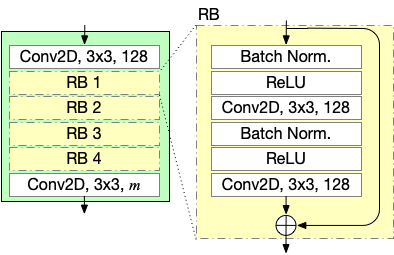
\includegraphics[scale=0.5]{BAB-2/resnet receiver.png}
    \caption{Arsitektur Blok ResNet}
    \label{fig:resnet}
\end{figure}